%%%%%%%%%%%%%%%%%%%%%%%%%%%%%%%%%%%%%%%%%%%%%%%%%%%%%%%%%%%%%%%%%%%%%
%
% Axel Fahy & Rudolf Höhn
% Spring Semester MSE
% MLBD
%
%%%%%%%%%%%%%%%%%%%%%%%%%%%%%%%%%%%%%%%%%%%%%%%%%%%%%%%%%%%%%%%%%%%%%%
%%%%%%%%%%%%%%%%%%%%%%%%%%%%%%%%%%%%%%%%%%%%%%%%%%%%%%%%%%%%%%%%%%%%%%%%%%%%%%%%
%2345678901234567890123456789012345678901234567890123456789012345678901234567890
%        1         2         3         4         5         6         7         8

%\documentclass[letterpaper, 10 pt, conference]{ieeeconf}  % Comment this line out
                                                          % if you need a4paper
\documentclass[a4paper, 10pt, conference]{ieeeconf}      % Use this line for a4
                                                          % paper

\IEEEoverridecommandlockouts                              % This command is only
                                                          % needed if you want to
                                                          % use the \thanks command
\overrideIEEEmargins
% See the \addtolength command later in the file to balance the column lengths
% on the last page of the document

% UTF8 support
\usepackage[utf8]{inputenc}
\usepackage[T1]{fontenc}

% The following packages can be found on http:\\www.ctan.org
\usepackage{graphics} % for pdf, bitmapped graphics files
%\usepackage{epsfig} % for postscript graphics files
%\usepackage{mathptmx} % assumes new font selection scheme installed
%\usepackage{times} % assumes new font selection scheme installed
\usepackage{amsmath} % assumes amsmath package installed
\usepackage{amssymb}  % assumes amsmath package installed
\usepackage{hyperref} % url links
\usepackage{hhline} % for more flexible lines in table
\usepackage[group-separator={,}, group-minimum-digits=4]{siunitx} % comma separator for number
\usepackage{dblfloatfix}
\usepackage{fixltx2e}

\graphicspath{{figures/}{./}} % Specifies where to look for included images

%-------------------------------------------------------------------------------
% TODONOTES
%-------------------------------------------------------------------------------
\usepackage{xargs}                  % Use more than one optional parameter in a new commands
\usepackage[dvipsnames]{xcolor}
\usepackage[colorinlistoftodos,prependcaption,textsize=tiny]{todonotes}
\newcommandx{\unsure}[2][1=]{\todo[linecolor=red,backgroundcolor=red!25,bordercolor=red,#1]{#2}}
\newcommandx{\change}[2][1=]{\todo[linecolor=blue,backgroundcolor=blue!25,bordercolor=blue,#1]{#2}}
\newcommandx{\info}[2][1=]{\todo[linecolor=OliveGreen,backgroundcolor=OliveGreen!25,bordercolor=OliveGreen,#1]{#2}}
\newcommandx{\improvement}[2][1=]{\todo[linecolor=Plum,backgroundcolor=Plum!25,bordercolor=Plum,#1]{#2}}
\newcommandx{\thiswillnotshow}[2][1=]{\todo[disable,#1]{#2}}

\title{\LARGE \bf
Race Prediction using a Long Short-Term Memory Model\\
\vspace*{0.05 in}
\small{Machine Learning on Big Data}
}

\author{ \parbox{3 in}{\centering Axel Fahy\\
         %\thanks{*Use the $\backslash$thanks command to put information here}\\
         {\tt\small axel.fahy@master.hes-so.ch}}
         \hspace*{ 0.5 in}
		 \parbox{3 in}{\centering Rudolf Höhn\\
         %\thanks{*Use the $\backslash$thanks command to put information here}\\
         {\tt\small rudolf.hohn@master.hes-so.ch}}
         \\\\
         \centering
         HES-SO//Master, Av. de Provence 6, 1007 Lausanne, Switzerland
%         \hspace*{ 0.33 in}
%		 \parbox{2 in}{\centering Andres Perez-Uribe\\
%         %\thanks{*Use the $\backslash$thanks command to put information here}\\
%         Laboratory of Intelligent Data Analysis\\
%         HES-SO//HEIG-VD\\
%         {\tt\small andres.perez-uribe@heigvd.ch}}
}

%\author{Axel Fahy and Rudolf Höhn}% <-this % stops a space

\begin{document}

\maketitle
\thispagestyle{empty}
\pagestyle{empty}

%%%%%%%%%%%%%%%%%%%%%%%%%%%%%%%%%%%%%%%%%%%%%%%%%%%%%%%%%%%%%%%%%%%%%%%%%%%%%%%%
\begin{abstract}
Connected devices such as smartwatches and fitness wristbands are getting more and more popular producing more and more data everyday. Runners use these devices to track all their movements. Using a Long Shot-Term Memory neural network, this paper shows that recurrent neural network can be used to keep in memory implicit features like the tiredness of a runner and predict his speed on a known path. The results show a small \textit{loss} in the training and evaluation process, however, when plotting the predicting run over the original run, the plots are quite different with few resemblances. The model is trained over a sample of runs and with a simple architecture with less than 200 parameters. Further work is required with the whole dataset available, on a longer period of time for the training phase and a more complex model.

\end{abstract}

%%%%%%%%%%%%%%%%%%%%%%%%%%%%%%%%%%%%%%%%%%%%%%%%%%%%%%%%%%%%%%%%%%%%%%%%%%%%%%%%
\section{INTRODUCTION}
Connected devices such as smartwatches and fitness wristbands are getting more and more popular producing more and more data everyday. These data allow the user to analyze their wellbeing, how they move and their performance, however all these are post-analysis. This paper presents a model that can be used to coach the user while he is running by predicting his speed. Knowing that, the application on his smartwatch or smartphone would be able to recommend the user to decrease or increase his pace to have a run in adequacy with the runner's objectives.

\section{DATA SOURCE}

Data come from different GPS running watches. It is composed of 30 different races. Each race is contained in a \texttt{.tab} file containing the time, the elevation, the distance and the speed. Sampling frequency is about 3 seconds between each data point, however, time between measures is not very precise. Due to some missing values in some data points, such as \textit{NA} values most of the time on the first line, these latter were removed and have not been taken into account. The number of samples by race is visible in Table~\ref{tbl:data-source}. As shown, races have between 418 and 860 points.

\begin{table}[thpb]
  \begin{center}
    \begin{tabular}{|c||c|}
    \hline
    \textbf{Race number} & \textbf{Number of points}\\
    \hline
    \hline
    Race=0 & 616\\
    Race=1 & 725\\
    Race=2 & 418\\
    Race=3 & 735\\
    Race=4 & 655\\
    Race=5 & 732\\
    Race=6 & 823\\
    Race=7 & 581\\
    Race=8 & 734\\
    Race=9 & 860\\
    Race=10 & 527\\
    Race=11 & 583\\
    Race=12 & 595\\
    Race=13 & 566\\
    Race=14 & 583\\
    Race=15 & 536\\
    Race=16 & 715\\
    Race=17 & 605\\
    Race=18 & 682\\
    Race=19 & 685\\
    Race=20 & 833\\
    Race=21 & 577\\
    Race=22 & 709\\
    Race=23 & 693\\
    Race=24 & 435\\
    Race=25 & 603\\
    Race=26 & 726\\
    Race=27 & 527\\
    Race=28 & 853\\
    Race=29 & 773\\
    \hline
    \end{tabular}
  \end{center}
  \caption{Number of points by race}
  \label{tbl:data-source}
\end{table}

Figure~\ref{fig:speed-slope} shows the values of the speed and the slope of one race of the dataset. As expected, when the slope is increasing, the speed is decreasing. The speed is a value that ranges around $2.0$ and $4.0 [m \cdot s^{-1}]$. The slope is between $-10\%$ and $10\%$.

\begin{figure*}[thpb]
  \center
  \centering
  \framebox{
    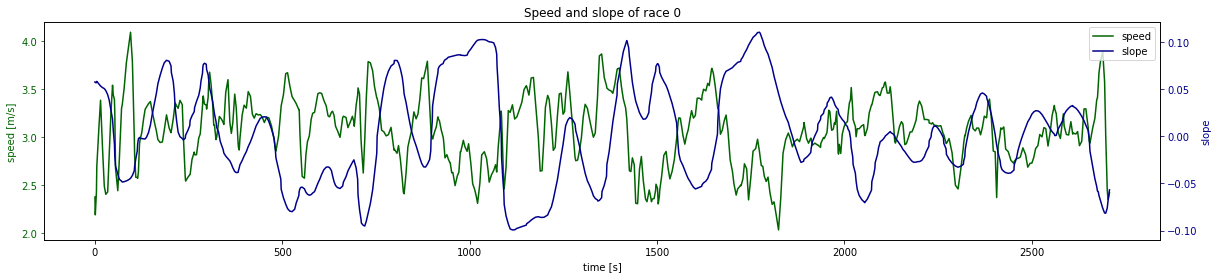
\includegraphics[scale=0.4]{03_plot_speed_slope.png}}
  \caption{Plot of speed and slope of race 0}
  \label{fig:speed-slope}
\end{figure*}

Figure~\ref{fig:elevation-distance} shows the elevation and the distance of the same race. The elevation is very different between the runs but within one run, the minimum and maximum values are separated by at most $200 [m]$. The distance is between $5,000 [m]$ and $10,000 [m]$. This is just an example of one race from the dataset, however, other races have similar data.

\begin{figure*}[thpb]
  \center
  \centering
  \framebox{
    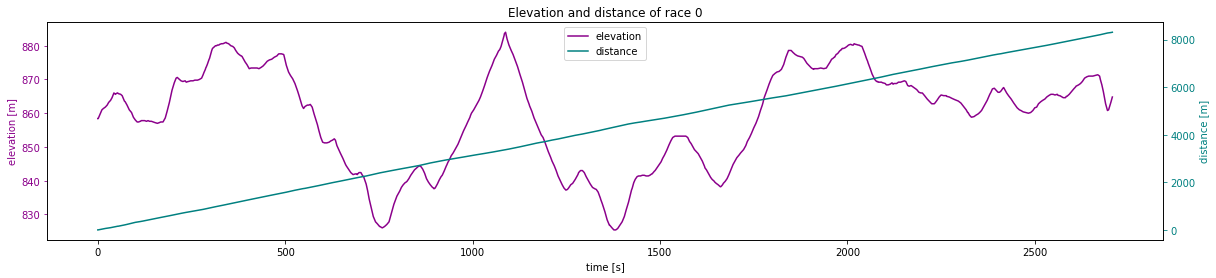
\includegraphics[scale=0.4]{04_plot_elevation_distance.png}}
  \caption{Plot of elevation and distance of race 0}
  \label{fig:elevation-distance}
\end{figure*}

Table~\ref{tbl:stats-dataset} describes the whole dataset. Statistical measure such as count, mean, standard deviation, quartile, maximal and minimal value are calculated.

Due to missing values (\textit{NA}), the count on every column is not the same. Data points with missing values have not been taken into account as they would not be meaningful. Moreover, since data have been collected in real life conditions, the dataset contains anomalies. For example, the maximal speed is $54.69[m \cdot s^{-1}]$ which is neither realistic nor even possible. This is because of a race that started with a speed abnormally high for a few data points before returning to standard values.

Considering that the final goal would be to execute the model in real time with real data, such anomalies, similar cases, might occur. This is why those irregularity have been left intact.

\begin{table}[h]
  \caption{Statistics on dataset}
  \begin{center}
    %\begin{tabular}{|l||*{5}{S[table-format=4.2]}}
    \begin{tabular}{|l||r|r|r|r|r|}
    \hhline{~-----}
    \multicolumn{1}{l|}{} & \textbf{Time} & \textbf{elevation} & \textbf{distance} & \textbf{speed} & \textbf{slope}\\
    \hhline{-=====}
    count & 19,691 & 19,685 & 19,685 & 19,685 & 19,691\\
    mean & 1,420.07 & 770.29 & 4,218.05 & 3.10 & 0.002\\
    std & 859.00 & 97.44 & 2,640.13 & 1.14 & 0.044\\
    min & 0.00 & 412.00 & 0.00 & 0.00 & -0.340\\
    25\% & 687.00 & 758.00 & 1,974.31 & 2.82 & -0.025\\
    50\% & 1,389.00 & 796.60 & 4,050.67 & 3.10 & 0.002\\
    75\% & 2,094.00 & 823.40 & 6,278.56 & 3.35 & 0.029\\
    max & 3,826.00 & 884.00 & 12,011.02 & 54.69 & 0.209\\
    \hline
    \end{tabular}
  \end{center}
  \label{tbl:stats-dataset}
\end{table}

\section{FEATURE EXTRACTION}

Given that the elevation and the distance of each point is provided, the slope is easily calculated and used as a feature.

The data have been normalized as follow. Running on all the training set, the highest and smallest values of each feature have been extracted. Afterwards, all the dataset has been normalized using a min-max scaling with the following formula: $X_{\textrm{norm}} = \frac{X - X_{\textrm{min}}}{X_{\textrm{max}} - X_{\textrm{min}}}$.

Data have been parsed in order to create the feature vector. Each one contains 10 data points with the 11$^{\text{th}}$ speed as target value. The feature vector also contains the slope of the 11$^{\text{th}}$ point. The model might need to know how the path is evolving to predict further speeds. The slope can also be the average slope of the next 5 or 10 points bringing less and more information at the same time.

Dataset has been shuffled in two different ways. Firstly, the order of the races of the dataset has been randomized, secondly, the data points within races have been shuffled to avoid creating bias in the training process.

The different combinations of these features are the main process of the model evaluation. The aim is to measure which features are valuable and which ones are redundant. For example, the slope already takes into consideration the elevation and the distance. Thus, it raises the question if elevation and distance are interesting features for the model.

\section{LONG SHORT-TERM MEMORY NEURAL NETWORK}

Long short-term memory (LSTM) is a recurrent neural network (RNN) specially developed to keep long-term dependencies without experiencing vanishing gradients \cite{lstm}.
LSTMs use gates to deal with input, output and memory cells.

The first gate, the forget gate, is a sigmoid function that varies between 0 and 1, representing respectively forget and remember totally the previous state. The input gate uses a sigmoid and hyperbolic tangent to choose if the model has to update the input value and with what. The memory is updated by the result of the forget and the input gate. The last gate is the output gate and its role is to output a value by taking into consideration the memory cell and the input value.

The aim of this project is to be able to predict the speed of a runner with implicit data like the tiredness. For this reason, the LSTMs were chosen because the model has to be able to remember the path the runner already ran (e.g. 100 meters of elevation within a short distance has not the same effect as 10 meters of elevation within a long distance).

Multiple hyper-parameters are possible. The first is the number of LSTM units used to construct the model. Hence, the number of LSTM units is part of the different model configuration that are tested in this paper. Other hyper-parameters are the choice of a loss function and of an optimizer. The time available for this project was short, thus these hyper-parameters have not been tested in the paper but taken for granted. The loss function chosen is the \textit{Mean Squared Error} (MSE). The optimizer is \textit{adam} \cite{adam}. Adam is a form of stochastic gradient descent (SGD) with the more powerful descent strategy than the original SGD.

The number of parameters of a LSTM depends on the shape of the feature vector and the output shape (i.e. the number of units) as shown in Equation \ref{equ:lstm} where $i$ referenced the input shape and $u$ the number of units.
\begin{equation}
\text{number of parameters} = 4 \cdot [(i + 1) \cdot u + u^2]
\label{equ:lstm}
\end{equation}

LSTMs are present in multiple domains such as machine translation \cite{machtran}, image captioning \cite{imacaption} or hand writing generation \cite{handwrite}.

\section{EXPERIMENTAL SETUP}

This section will present the different experimentations done in order to find the best model. The first run was done with all the basic features, namely the time, the elevation, the distance, the speed and the slope with 4 LSTM units and a batch size of 10. From this point, the goal was to adapt the features and the parameters of the model in order to obtain a better performance. During those experiments, each model has been trained on 20 races and tested with 10 races.

The first hypothesis was that some features were giving the same information and were not needed in the input vector. For example, the slope is created with the distance and the elevation of the current point with the ones from the last point. Therefore, the slope and the elevation for example can be considered as similar information and it may not be necessary to have both. Removing the elevation resulted in a better \textit{loss} and a \textit{val\_loss} value almost similar.

The second hypothesis was that the same principle could be applied for the distance and the time. Both features are represented in the speed, since the speed is the distance traveled within a given time. Removing the distance improved the performance, however, this was not the case regarding the time.

At this point, the best model was the one using the time, the speed and the slope as features. Given that the slope of the entire course of the race is known, the slope of the next point, the one with the speed being predicted, has been added in the input vector. Since the LSTM has the 10 last point as input vector, the value of the next slope had to be added in each of the previous points. The addition of this feature decreased the \textit{val\_loss} of $0.0007$.

With those features in mind, the next step was to alter the parameters of the model to observe if performance could be even better. The batch size and the number of LSTM units were the main parameters that could influence the results. The number of epochs could also be modified, but given that with 100 epochs the model had already converged, there was no point in increasing it.

A batch size of 1 and 100 have been tried with the previous features, the one that gave the best results so far was with a size of 10. The number of LSTM units has been increased to 8, 16 and 32 LSTM units.

Another experimentation was to change the goal of the prediction. Instead of predicting only the next speed, the prediction has be done on the average of the next 5 speeds.

\section{RESULTS \& DISCUSSION}

Table~\ref{tbl:result-by-technique} shows the results of the different experiments explain in the previous part. All the experiments are doing 100 iterations, the \textit{loss} and \textit{val\_loss} values are the ones at the 100$^{\textrm{th}}$ iteration. A batch size of 10 and 4 LSTM units were used unless specified otherwise in the description. Each of the results from Table~\ref{tbl:result-by-technique} are available on GitHub\footnote{\url{https://github.com/axelfahy/RacePrediction}} under a tag, being the same as in the table. Each result are presented in a Jupyter Notebook, allowing to compare and keep an historic of all experiments.

\begin{table}[h]
  \caption{Performance of each experiment}
  \begin{center}
    \begin{tabular}{|l||c|c|}
    \hline
    \textbf{Experiment} & \textbf{loss} & \textbf{val\_loss}\\
    \hline
    \hline
    A=feat.time-elevation-distance-speed-slope & 0.0603 & 0.0280\\
    B=feat.time-distance-speed-slope & 0.0591 & 0.0281\\
    C=feat.time-speed-slope & 0.0587 & \textbf{0.0278}\\
    D=feat.distance-speed-slope & 0.0551 & 0.0318\\
    E=feat.speed-slope & 0.0593 & 0.0287\\
    \textbf{F=feat.time-speed-slope-slopeNext} & 0.0589 & \textbf{0.0271}\\
    G=feat.time-speed-slope-slopeNext-avg5 & 0.0837 & 0.0519\\
    H=feat.time-speed-slope-slopeNext-batch1 & 0.0575  & 0.0345\\
    I=feat.time-speed-slope-slopeNext-batch100 & 0.1017 & 0.0455\\
    J=feat.time-speed-slope-slopeNext-units8 & \textbf{0.0532} & \textbf{0.0278}\\
    K=feat.time-speed-slope-slopeNext-units16 & 0.0415 & 0.0306\\
    L=feat.time-speed-slope-slopeNext-units32 & \textbf{0.0391} & 0.0322\\
    \hline
    \end{tabular}
  \end{center}
  \label{tbl:result-by-technique}
  \medskip
  \small
  \textbf{A}: Features: time, elevation, distance, speed and slope / \textbf{B}: Same as A, but without the elevation / \textbf{C}: Same as B, but without the distance / \textbf{D}: Same as B, but without the time / \textbf{E}: Only speed and slope as features / \textbf{F}: Same as C, but with the value of the next slope added / \textbf{G}: Same as F, but with the average of the 5 next slopes and trying to predict the average of the 5 next speeds instead of 1 / \textbf{H}: Same as F, but with batch size of 1 instead of 10 / \textbf{I}: Same as F, but with batch size of 100 / \text{J}: Same as F, but with 8 LSTM units instead of 4 / \textbf{K}: Same as F, but with 16 LSTM units / \textbf{L}: Same as F, but with 32 LSTM units.
\end{table}

% figure* environment allows the figure to be put on all the width of the page.
\begin{figure*}[h]
  \center
  \centering
  \framebox{
    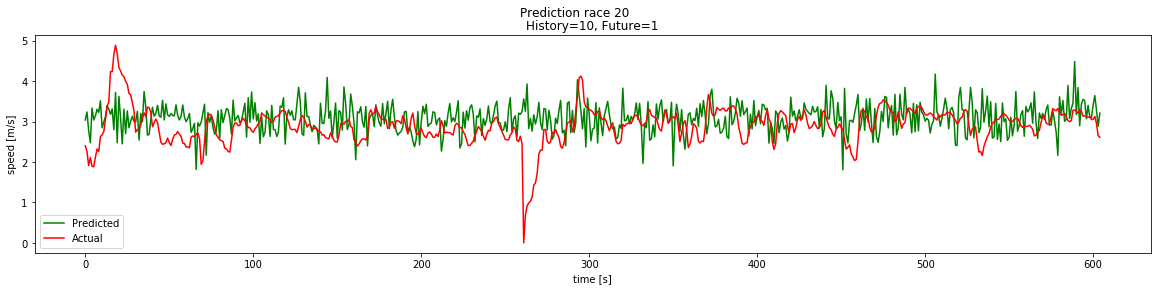
\includegraphics[scale=0.4]{02_plot_feat_time_speed_slope_slopeNext.png}}
  \caption{Plot of a race with its prediction}
  \label{fig:plot-race}
\end{figure*}

The best model is the F, using the time, the speed, the slope and the value of the next slope with a batch size of 10 an 4 LSTM units. It has been found after multiple experiments and chosen for three reasons. The determining metric is the \textit{val\_loss} and compared to more complex models presenting similar performance, the more complex were not chosen because it also means a longer training phase and higher risk of experiencing overfitting.

It was an iterative process with only one modification at a time in order to observe the impact of the current experiment. The modification of the batch size did not improve the performance. A small value increased the execution time but did not perform better.

Increasing the number of LSTM units could be a possibility for future experiments. Indeed, with 32 LSTM units, the \textit{loss} value was the smallest, however, the \textit{val\_loss} was higher than expected.

The Figure~\ref{fig:plot-race} shows the plot of an actual race (in red) compare to the prediction (in green). The prediction is not exactly in harmony with the real speed of the race. However, there are still some similarities.

The Figure~\ref{fig:score-lstm} shows a plot of the results of the training and testing set. After 50 epochs, the results are stabilizing and stop moving much, except for some fluctuations. The testing is better than the training, so the model does not suffer of overfitting.

\begin{figure}[thpb]
  \centering
  \framebox{
    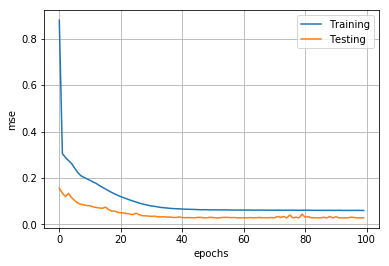
\includegraphics[scale=0.5]{01_score_feat_time_speed_slope_slopeNext.png}}
  \caption{Results of training and testing}
  \label{fig:score-lstm}
\end{figure}

\section{Conclusion}

This paper showed that using an LSTM for speed prediction in a race could be a possibility. More experiments could be undertaken to improve the performance of the system and have a better prediction of the race's speed.

\addtolength{\textheight}{-12cm}   % This command serves to balance the column lengths
                                  % on the last page of the document manually. It shortens
                                  % the textheight of the last page by a suitable amount.
                                  % This command does not take effect until the next page
                                  % so it should come on the page before the last. Make
                                  % sure that you do not shorten the textheight too much.

%%%%%%%%%%%%%%%%%%%%%%%%%%%%%%%%%%%%%%%%%%%%%%%%%%%%%%%%%%%%%%%%%%%%%%%%%%%%%%%%
\begin{thebibliography}{99}

\bibitem{lstm} Sepp Hochreiter and Jürgen Schmidhuber (1997). Long Short-Term Memory. Neural Computation, 9, 1735-1780.
\bibitem{adam} Diederik P. Kingma and Jimmy Ba (2014). Adam: A Method for Stochastic Optimization. CoRR, abs/1412.6980.
\bibitem{machtran} Ilya Sutskever and Oriol Vinyals and Quoc V. Le(2014). Sequence to Sequence Learning with Neural Networks. CoRR, abs/1409.3215.
\bibitem{imacaption} Oriol Vinyals and Alexander Toshev and Samy Bengio and Dumitru Erhan(2014). Show and Tell: A Neural Image Caption Generator. CoRR, abs/1411.4555, .
\bibitem{handwrite} Alex Graves (2013). Generating Sequences With Recurrent Neural Networks. CoRR, abs/1308.0850.
\end{thebibliography}

%-------------------------------------------------------------------------------
% TABLE WITH TODOLIST
%-------------------------------------------------------------------------------
%\listoftodos[Notes]

\end{document}
